\documentclass{article}

\usepackage[final]{neurips_2020}
\usepackage[utf8]{inputenc} % allow utf-8 input
\usepackage[T1]{fontenc}    % use 8-bit T1 fonts
\usepackage{hyperref}       % hyperlinks
\usepackage[pdftex]{graphicx}
\usepackage{url}            % simple URL typesetting
\usepackage{booktabs}       % professional-quality tables
\usepackage{amsfonts}       % blackboard math symbols
\usepackage{nicefrac}       % compact symbols for 1/2, etc.
\usepackage{microtype}      % microtypography
\usepackage[usenames,dvipsnames]{color}

\title{Magneto-optical Kerr effect and magnetic anisotropy}

\author{
Umur Can Kaya\\
5410770\\
\texttt{umurcan.kaya@gmail.com}\\
\And
Rohit Sharma\\
5442717\\
\texttt{rohis97@zedat.fu-berlin.de}\\
}

\begin{document}

\maketitle

\begin{abstract}
In this experiment we utilized magneto-optical Kerr effect (MOKE) to obtain information about the magnetic properties of bcc-Fe film. 
\end{abstract}

\section{Introduction}
The magneto-optical Kerr-effect (MOKE) allows us to optically read out the magnetic properties of ferro magnets. MOKE signal is said to be proportional to the sample magnetization and allows us to read out MOKE hysteresis loops which gives us information on physical quantities such as coercitivity, remanence that can also be calculated. We use longitudal MOKE, to measure the magnetic properties of a thin bcc-Fe (001) single crystal. We "see"  domain pattern of a rare-earth iron garnet film using Polar Kerr microscope. Because of these properties MOKE has wide applications and has generated wide interest. 
\subsection{Magneto-optical Kerr effect}
When light passes through  matter whose  magnetic dipoles are aligned the reflection of this light gives away a change in polarization direction (Kerr-rotation) and  ellipticity which we can observe. These effects are explained by quantum mechanics namely spin orbit interaction which is the dynamic of the motion of the particle relative to it's spin.

\subsection{Magnetic anisotropy}
Magnetic Anisotropy refers to the dependence of  magnetic properties on direction. This is explained by spin orbit coupling and magnetic dipole interaction. Certain directions are energetically (minimum energy required) preferred over others for magnetization and these are called easy axes. Hard axes are those directions where  higher energy is required for magnetization. In this experiment there are two different causes of magnetic anistropy - Crystal and Shape anisotropy.
\subsubsection{Crystal anisotropy}
Due to crystal anisotropy, it takes different amount of energy to magnetize the crystal in certain directions than in others. This is caused by the magnetic dipole-dipole interaction or spin-orbit coupling. The crystal anisotropy energy per unit volume in cubic crystals is given as 
\begin{equation}
    E_\text{cryst} = K_0 + K_1(\alpha_1^2\alpha_2^2 + \alpha_2^2\alpha_3^2 + \alpha_1^2\alpha_3^2) + K_2(\alpha_1^2\alpha_2^2\alpha_3^2) + \cdots
\end{equation} 
where $K_1,\ K_2,\ K_3$ are crystal anisotropy constants that depends on the material and the temperature. $\alpha_1,\ \alpha_2,\ \alpha_3$ are the cosine values of the angles of the direct lattice vectors. In many cases, compared to $K_0$ and $K_1$, $K_s$ with $s>1$ are small enough to be neglected.
\begin{equation}
    E_\text{cryst} \simeq K_0 + K_1(\alpha_1^2\alpha_2^2 + \alpha_2^2\alpha_3^2 + \alpha_1^2\alpha_3^2)
\end{equation} 
From this we can calculate the crystal anisotropy energy for magnetization directions as\\
\begin{center}
\begin{equation}
E_\text{cryst} = \left\{
        \begin{array}{ll}
            K_0, & \quad[100]\\
            K_0 + \frac{K_1}{4}, &\quad [110]
        \end{array}
    \right.
\end{equation}    
\end{center}
The difference between two directions can be calculated as $\Delta E = K_1 / 4$.
\subsubsection{Shape anisotropy}
Shape anisotropy is caused by the shape of the sample, with the energy given as
$$ E_\text{shape} = \frac{\mu_0}{2}H_DM_S = \frac{\mu_0}{2}NM_S^2$$
where $M_S$ is the saturation magnetization and $N$ is the demagnetization factor which depends on the magnetization direction.
\subsection{Hysteresis loops}
Magnetic hysteresis is dipole alignment. For different low values of external magnetic fields the sample is not magnetized homogeneously (for thin films or small samples).\\

B increases as much as H increases following the the curve I , as shown in Fig. This trend is called first magnetization curve. \\
From a certain value of H , $H_m$ , B starts to increase proportionally to $µ_0$ H. This means that for H = $H_m$ intensity magnetization reaches its maximal 
value M = $M_s$ , called saturation point.\\
We start to decrease H ,the   curve   B(H) follows the same  curve  I but in  the  opposite  direction. \\
For H = 0, B assumes what is usually called remenence value Br , and M as well, M = $B_r$ /$µ_0$ , is called remanence magnetization.
5) Inverting the sign of H and increasing its absolute value B and M start to decrease. For H = $−H_c$ we have B = 0. $H_c$ is called magnetic coercivity. \\
For H  < $−H_c$ , B  starts to be negative too. The complete 
curve  is  also  known  as  hysteresis  curve. \\

\subsection{Magnetic domains}
A ferromagnetic sample in remanence builds up a magnetic domain pattern. Each domain is spontaneously magnetized to the saturation value $M_s$ , but 
the directions of magnetization of the various domains are such that the material has no net magnetization. Parallel alignment of all magnetic moments preferably results in stray fields. Furthermore the building of domain structures (Néel and Bloch walls) consumes energy. Magnetization consists in aligning all the different domains in the sample into a single domain state magnetized in the same direction as the applied external field. Therefore the domain pattern is regulated by the minimum of the total energy, which is a combination of exchange interaction, stray field energy, crystal anisotropy and Zeeman energy. The rare-earth iron garnet film examined in this experiment has a maze domain structure with a constant domain width in the r.
\clearpage
\section{Experimental setup}
\subsection{Magneto-optical Kerr effect}
The experimental setup is shown in figure \ref{fig:exp_setup}. The Fe[110] film is placed inside the ring shaped iron core which is winded by a coil. The external magnetic field experienced by the sample can be controlled by adjusting the current passing through the coil. This magnetic field can be measured by using a Hall-probe. The sample can be rotated around [001] and magnetized along different directions, [100] and [110] in our case. A linearly polarized He-Ne laser of output power 0.5 mW is used as the light source. The laser beam reflected of the surface of the sample passes through a the analyzer before hitting the photo diode. The signal from the photodiode is then amplified and converted to digital to be read out by the computer. Kerr rotation can be measured indirectly by reading off the intensity at different analyzer orientations.
\begin{figure}[h!]
\centering
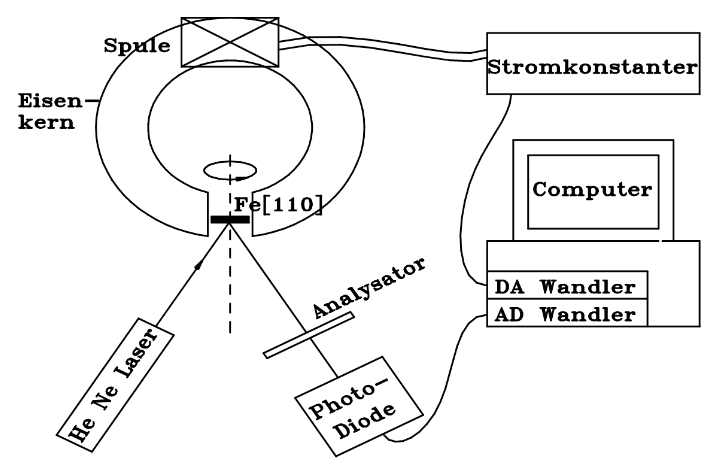
\includegraphics[width=0.6\linewidth]{LAB/MOKE/experimental_setup.PNG}
\caption{Sketch of the experimental setup for MOKE.}
\label{fig:exp_setup}
\end{figure}
\subsection{Kerr microscope}
A Kerr microscope, which utilizes polar MOKE geometry, is used to visualize the magnetic domains of the rare-earth metal. The microscope is equipped with a charge-coupled device (CCD) camera that converts the light reflected from the sample to electronic signal. The external magnetic field which the sample is being subjected to is generated by an electromagnet.
\clearpage
\section{Tasks}
\subsection{Magnetic field calibration}
Using Ampere's circuital law  \\
\begin{equation}
    \oint \vec{B}.\vec{ds} = \mu_{0}NI
\end{equation}
N is number of coil windings and I is the current. \\
\begin{equation}
\frac{B(2\pi r - w) }{\mu_{1}/\mu_{0}} + \frac{Bw}{\mu_{2}/\mu_{0}} = NI
\end{equation}
where $\mu_1$/$\mu_0$ = 5000 is the relative permeability of the 
circular iron core and $\mu_2$/$\mu_0$ = 1 is the air permeability, w is 
the width of the sample and r is the radius of the iron core. 
Since $\mu_1$/$\mu_0$ = 5000 and we want a linear relation among 
B and I we are allowed to neglect the first term.
\begin{equation}
B = \frac{NI}{w} = 0.0314 I.    
\end{equation}
We used a Hall probe to measure the magnetic field at the position of the sample to measure the linear relation of $B$ and $I$. Measured data with the best fit line is given in the figure. The relation we obtain was:
\begin{equation}
    B =  0.00626 I - 0.00002
\end{equation}

\begin{figure}[h!]
\centering
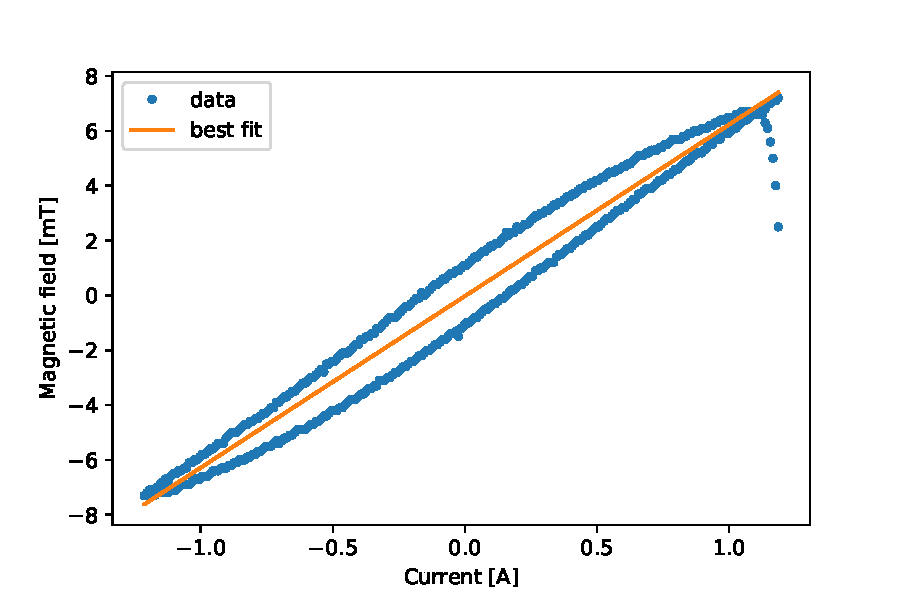
\includegraphics[width=0.7\linewidth]{LAB/MOKE/calibration.pdf}
\caption{Calibration data.}
\label{fig:exp_setup}
\end{figure}

\clearpage
\subsection{Magnetic anisotropy}

\begin{figure}[h!]
\centering
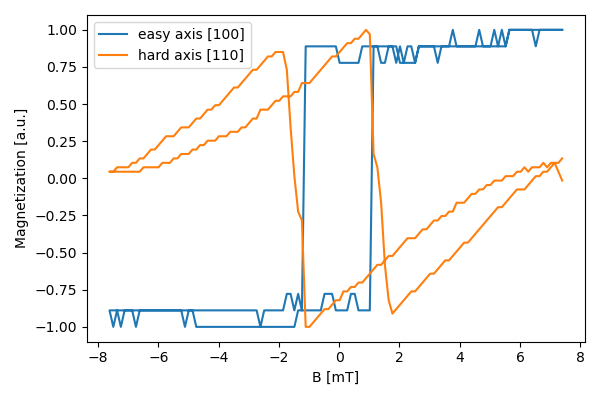
\includegraphics[width=0.7\linewidth]{LAB/MOKE/hysteresis.png}
\caption{Hysteresis loops for easy and hard axes.}
\label{fig:exp_setup}
\end{figure}

\clearpage
\subsection{Contrast and Kerr rotation}
Magnetic contrast is given by
\begin{equation}
c = \frac{I_{+} - I_{-}} {I_{0}} = 2  \frac{I_{+} - I_{-}} {I_{+} + I_{-}}
\end{equation}
where $I_{+}$ and $I_{-}$ are saturation signals for both directions of magnetic field. $I_{0}$ is average intensity. Malus law for a light passing through a analyzer gives the intensity as follows
\begin{equation}
I_{trans} = I_{i} cos^2 \theta 
\end{equation}
where $I_{trans}$ is intensity of light transmitting the sample $I_{i}$ and $\theta$ is the angle between the analyzer and the initial direction of polarization.In the experiment we are measuring the reflected beam, we can write the measured intensity in the following form
\begin{equation}
I_{ref} = I_{i} sin^2 \theta
\end{equation}
Using this, magnetic contrast can be written as
$$ c = 2\frac{sin^2(\theta_+) - sin^2(\theta_-)}{sin^2(\theta_+) + sin^2(\theta_-)} $$
If we write the saturation angles in terms of analyzer position $\alpha$ and Kerr rotation $\Theta_K$ we get
$$ c = 2\frac{sin^2(\alpha + \Theta_K) - sin^2(\alpha - \Theta_K)}{sin^2(\alpha + \Theta_K) + sin^2(\alpha - \Theta_K)} $$
Small angle approximation for $\alpha$ and $\Theta_K$ gives
$$ c = \frac{4\alpha\Theta_K}{\alpha^2+\Theta^2_K} \simeq \frac{4\Theta_K}{\alpha}.$$
Given the analyser position, by measuring magnetic contrast we can calculate the Kerr angle.

\begin{figure}[h!]
\centering
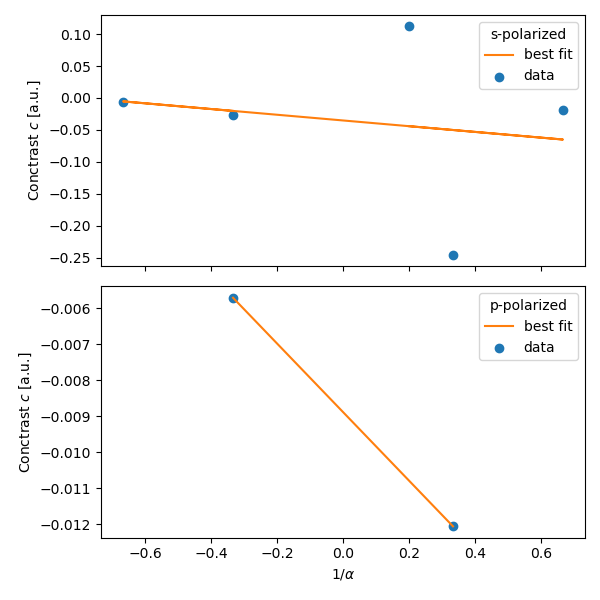
\includegraphics[width=0.6\linewidth]{LAB/MOKE/kerr_rotation.png}
\caption{Kerr rotation vs 1/$\alpha$ for s and p polarized light.}
\label{fig:exp_setup}
\end{figure}

\begin{table}[]
\centering
\begin{tabular}{|l|l|l|}
\hline
           & s-polarized & p-polarized \\ \hline
Literature & -0.699      & 0.0848      \\ \hline
Experiment & -0.011      & -0.0024     \\ \hline
\end{tabular}
\end{table}

\clearpage
\subsection{Kerr microscopy}   
We were provided with Kerr microscopy images given in the figure. By integrating the intensities over all pixels we obtain the following figure.

\begin{figure}[h!]
\centering
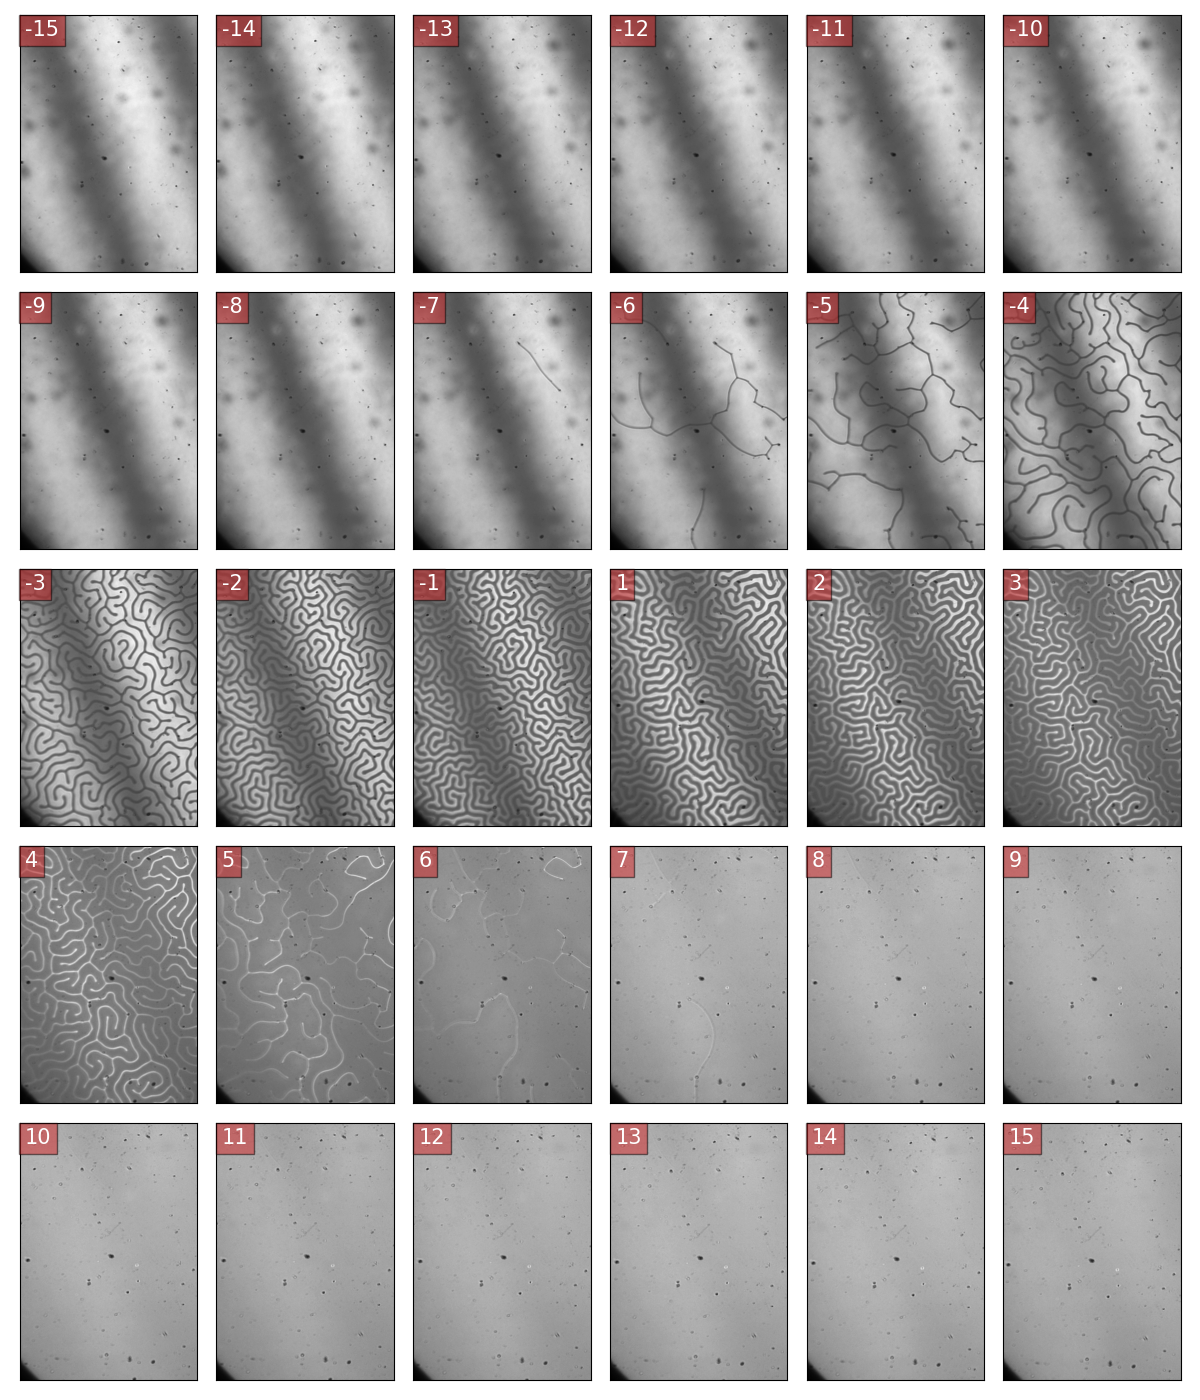
\includegraphics[width=0.8\linewidth]{LAB/MOKE/domains.png}
\caption{Kerr microscopy images.}
\label{fig:exp_setup}
\end{figure}

\begin{figure}[h!]
\centering
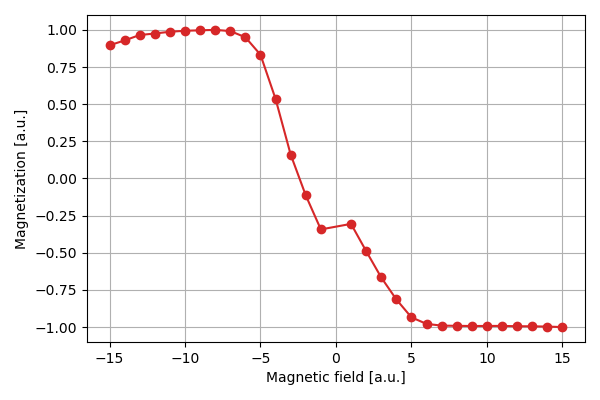
\includegraphics[width=0.6\linewidth]{LAB/MOKE/kerr_mic_loop.png}
\caption{Integrated Kerr microscopy intensities.}
\label{fig:exp_setup}
\end{figure}

\clearpage
\section{Discussion}
We used Magneto-optical Kerr effect to obtain information about the magnetic properties of the material. In the first task we calculated the calibration factor of the external magnetic field related to the current passing through the coil. We measured a hysteresis instead of a linear relation which indicates a ferromagnetic Gaussmeter probe. In the second task we measured the magnetization of the sample at different directions to calculate the crystal anisotropy constants of the sample. As seen in the relevant figure the difference between easy and hard axes is clear but due to the unexpected shape of the hysteresis loop for the hard axes, we couldn't proceed with the calculations. In the third part, we measured the magnetization for different analyzer angles aiming to calculate the Kerr rotation. Our results differ from the literature values.
\section*{References}

[1] https://wiki.physik.fu-berlin.de/fp/lib/exe/fetch.php?media=private:ma12 instructions.pdf

[2] Kittel, Charles. 2004. Introduction to Solid State Physics. 8th ed. New York, NY: John Wiley & Sons.

[3] 

\end{document}
